
%\RequirePackage{pdf15}

\documentclass{beamer}

\usepackage[utf8]{inputenc}

\usepackage{mystyle}

\usepackage{tikz}
\usepackage{pgfplots}
\usepackage{subcaption}

\usepackage{natbib}
\bibliographystyle{apalike}
%\usepackage[style=authortitle,backend=biber]{biblatex}
%\addbibresource{anthology.bib}
%\addbibresource{emnlp2020.bib}
\renewcommand{\footnotesize}{\scriptsize}

\newcommand{\bigCI}{\mathrel{\text{\scalebox{1.07}{$\perp\mkern-10mu\perp$}}}}

\usepackage{tikz-dependency}
\usetikzlibrary{shapes.arrows, positioning, fit, bayesnet,
    arrows,backgrounds,patterns,matrix,calc,shadows,plotmarks,
    shapes,positioning,automata,positioning,spy,scopes,chains,decorations,decorations.pathreplacing}

\newcommand{\FancyUpArrow}{
\begin{tikzpicture}[baseline=-0.3em]
\node[single arrow,draw,rotate=90,single arrow head extend=0.2em,inner
ysep=0.2em,transform shape,line width=0.05em,top color=green,bottom color=green!50!black] (X){};
\end{tikzpicture}}
\newcommand{\FancyDownArrow}{
\begin{tikzpicture}[baseline=-0.3em]
\node[single arrow,draw,rotate=-90,single arrow head extend=0.2em,inner
ysep=0.2em,transform shape,line width=0.05em,top color=red,bottom color=red!50!black] (X){};
\end{tikzpicture}}

\AtBeginSection[]{
  \begin{frame}
  \vfill
  \centering
  \begin{beamercolorbox}[sep=8pt,center,shadow=true,rounded=true]{title}
    \usebeamerfont{title}\insertsectionhead\par%
  \end{beamercolorbox}
  \vfill
  \end{frame}
}

% quotes
\usepackage[style=british]{csquotes}

\def\signed #1{{\leavevmode\unskip\nobreak\hfil\penalty50\hskip1em
  \hbox{}\nobreak\hfill #1%
  \parfillskip=0pt \finalhyphendemerits=0 \endgraf}}

\newsavebox\mybox
\newenvironment{aquote}[1]
  {\savebox\mybox{#1}\begin{quote}\openautoquote\hspace*{-.7ex}}
  {\unskip\closeautoquote\vspace*{1mm}\signed{\usebox\mybox}\end{quote}}

%Information to be included in the title page:
\title{Word Games}
\author{J Chiu}

\setbeamertemplate{navigation symbols}{} 
\setbeamertemplate{footline}[frame number]

\begin{document}

\begin{frame}[plain]
\titlepage
\end{frame}

\begin{frame}
\frametitle{Dialogue and information gathering}
\begin{itemize}
\item Resolve ambiguity and coordinate through dialogue
\item OneCommon: Interactive, symmetric reference game
    \begin{itemize}
    \item Isolates info gathering (and coordination)
    \item Environment (dots) are completely static
    \item Dynamism comes from dialogue only
    \end{itemize}
\item 20 questions with symmetric information constraints
\end{itemize}
\end{frame}

\begin{frame}
\frametitle{Previous SotA}
\begin{itemize}
\item Purely supervised
    \begin{itemize}
    \item 
    \end{itemize}
\item Uncalibrated beliefs: overconfidence
    \begin{itemize}
    \item Pushes for to select a dot that will not work
    \end{itemize}
\item Research goal: Improve purely supervised models via model-based planning
\end{itemize}
\end{frame}


\begin{frame}
\frametitle{Fixing strategy with planning}
\begin{itemize}
\item Prior: Fully supervised neural encoder-decoder
    \begin{itemize}
    \item Encode past interactions with a neural net
    \item Generate what to say with a neural net
    \item Brittle strategy, less brittle language
    \end{itemize}
\item Next: Model-based planning
    \begin{itemize}
    \item Choose what to say by imagining how partner would respond
    \item Say utterance with best expected outcome
    \item Potentially stronger player than expert demonstrations
    \end{itemize}
\end{itemize}
\end{frame}

\begin{frame}
\frametitle{Challenges in model-based planning}
\begin{itemize}
\item Partner modeling is hard
    \begin{itemize}
    \item Variable amount of information
    \item Random strategies
    \end{itemize}
\item Multi-turn planning
    \begin{itemize}
    \item Accuracy of planning depends greatly on the partner model
    \item Errors from the partner model will compound over time
    \end{itemize}
\item Single-turn planning
    \begin{itemize}
    \item Removes compounding errors
    \item Optimize a dialogue progress heuristic: uncertainty reduction
    \item Requires belief
    \end{itemize}
\item Use what dots partner also sees as belief
\end{itemize}
\end{frame}

\begin{frame}
\frametitle{Planning}
\begin{itemize}
\item Plan by imaging partner response
$$\max_{u} \Es{p(r \mid h, u)}{\text{Utility}(h, u, r)}$$
\item Utterance $u$, response $r$, history $h$
\item Utility should approximate dialogue progress
    \begin{itemize}
    \item Goal of dialogue is information gathering and coordination
    \item Focus on information gathering
    \end{itemize}
\item Utility a function of belief
\end{itemize}
\end{frame}

\begin{frame}
\frametitle{Planning with Belief}
\begin{itemize}
\item Introduce belief state $p(s \mid h)$
    \begin{itemize}
    \item State $s$ is what dots partner can also see
    \end{itemize}
\item Incorporate belief in planning
$$\max_{u} \Es{p(r \mid h, u, s)p(s \mid h)}{\text{Certainty}(p(s \mid h, u, r))}$$
\item Obtain
$$p(s \mid h, u, r) = \frac{p(r \mid h, u, s)p(s \mid h)}{\sum_s p(r\mid h,u,s)p(s \mid h)}$$
\end{itemize}
\end{frame}

\begin{frame}
\frametitle{Belief model}
\begin{itemize}
\item Static latent quantity $y$: which dots do they also see
    \begin{itemize}
    \item Alternative: actual field of view
    \end{itemize}
\item Actions $a_t$, observations $o_t$
    \begin{itemize}
    \item Prior work: yes/no questions (20 questions)
    \item OneCommon: unrestricted language for both
    \end{itemize}
\item Uniform prior $p(y)$ over 7 choose 4 dots partner also sees
\item Observation model $p(o_t \mid a_{1:t-1},o_{1:t-1}, y)$
    \begin{itemize}
    \item Pick $y$ that is observed during training
    \item Ideally fully supervised
    \item Prior work\footnote{\citet{yu,padmakumar}}
        makes naive Bayes assumption $p(o_t \mid a_t, y)$ 
    \end{itemize}
\begin{center}
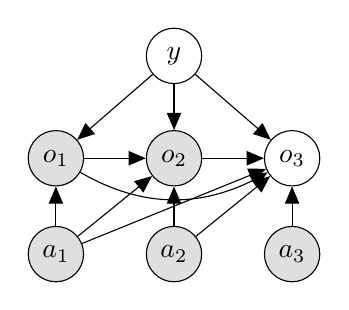
\begin{tikzpicture}
\node[latent] (y) {$y$};
\node[obs] at (-1.5,-1.3) (o1) {$o_1$};
\node[obs] at (0, -1.3) (o2) {$o_2$};
\node[latent] at (1.5,-1.3) (o3) {$o_3$};

\node[obs, below=.5cm of o1] (a1) {$a_1$};
\node[obs, below=.5cm of o2] (a2) {$a_2$};
\node[obs, below=.5 of o3] (a3) {$a_3$};

\edge {y} {o1};
\edge {y} {o2};
\edge {y} {o3};

\edge {a1} {o1};
\edge {a1} {o2};
\edge {a1} {o3};
\edge {a2} {o2};
\edge {a2} {o3};
\edge {a3} {o3};

\edge {o1} {o2};
\path (o1) edge[->, bend right=30] (o3);
\edge {o2} {o3};
\end{tikzpicture}
\end{center}
\end{itemize}
\end{frame}


\begin{frame}
\frametitle{Belief update}
\begin{itemize}
\item Interaction history $h_t = (a_0,o_0,\ldots,a_t,o_t)$
    contains all previous actions and observations
\item Given an initial belief $p(y \mid h_t)$ + next action/observation,
    obtain next belief via
    $$p(y \mid h_t, a_{t+1},o_{t+1})
    \propto \underbrace{p(o_{t+1} \mid h_t, a_{t+1}, y)}_{\text{observation model}}p(y\mid h_t)$$
\item Belief calibration depends on accuracy of observation model
\end{itemize}
\end{frame}

\begin{frame}
\frametitle{Observation model}
\begin{itemize}
\item Example exchange
    \begin{itemize}
    \item Action: Do you see a red dot?
    \item Observation: No, but I see a blue one.
    \end{itemize}
\item Utterances are multifaceted
    \begin{itemize}
    \item Responses contain more information than asked
    \item New information injected by partner due symmetric roles
    \item Very difficult to model new information
    \end{itemize}
\item Simplifying assumption: only model response, not new information
    \begin{itemize}
    \item Update belief state afterwards by pretending we asked corresponding question
    \item Allows reduction to 20 questions / assymetric role
    \end{itemize}
\item Supervised training needs observed $o,h,a,y$
    \begin{itemize}
    \item Main question: How to extract responses $o$?
    \end{itemize}
\end{itemize}
\end{frame}

\begin{frame}
\frametitle{Response extraction}
\begin{itemize}
\item Heuristic: Use repeated mentions from response
    \begin{itemize}
    \item Do you see a red dot? Yes, the one next to the blue one?
    \end{itemize}
\item Generalization: TBD
\item Recap: we have
    \begin{itemize}
    \item Belief over shared dots $p(y\mid h)$
    \item Observation model $p(o \mid h,a,y)$
    \item Update $p(y\mid h, a, o)$
    \item Reduced to assymmetric case by extracting response only
    \end{itemize}
\item Next: Single-turn planning
\end{itemize}
\end{frame}

\begin{frame}
\frametitle{Planning: Use prior work in assymmetric setting}
\begin{itemize}
\item Given history $h$,
we need to chose an action $a$ by optimizing heuristic utility
\begin{equation*}
\max_a U(h, a)
\end{equation*}
\item Utility $U$ = information gain - utterance - pragmatic cost
    \begin{itemize}
    \item IG: Reduce uncertainty
    \item Utterance cost: Can't send a full paragraph
    \item Pragmatic cost: Want utterance to be accurate
    \end{itemize}
\item Ideally would estimate and optimize future reward directly
    \begin{itemize}
    \item Heuristic approximation of future reward $U$
    \item Limited-horizon planning to minimize impact of model error
    \end{itemize}
\end{itemize}
\end{frame}

\begin{frame}
\frametitle{Expected information gain}
\begin{itemize}
\item Maximizing expected information gain equivalent to minimizing uncertainty
$$\min_a \sum_o\sum_y
    \underbrace{p(o\mid h,a,y)}_{\text{observation model}}
    \underbrace{p(y\mid h)}_{\text{belief}}
    \text{Uncertainty}(\underbrace{p(y \mid h,a,o)}_{\text{new belief}})$$
\end{itemize}
\end{frame}

\begin{frame}
\frametitle{Summary}
\begin{itemize}
\item Goal: Extend methods from 20 questions to symmetric, language setting
\item Extract relevant information from partner utterances
\item Use explicit belief state + single-turn planning heuristic
\end{itemize}
\end{frame}

\begin{frame}
\frametitle{End}
\end{frame}

\begin{frame}
\frametitle{Information Gain}
\begin{itemize}
\item A good action should decrease uncertainty
\item Requires
    \begin{itemize}
    \item Belief distribution over selection item given history $p(y \mid h)$
    \item Partner response model $p(o \mid h, a, y)$
    \end{itemize}
\item Represent a turn as
\begin{center}
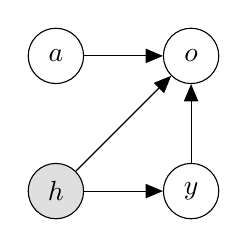
\begin{tikzpicture}
\node[obs] (h) {$h$};
\node[latent, right=of h] (i) {$y$};
\node[latent, above=of i] (o) {$o$};
\node[latent, above=of h] (a) {$a$};
\edge {h} {i};
\edge {h} {o};
\edge {i} {o};
\edge {a} {o};
\end{tikzpicture}
\end{center}
\item Language and planning coupled
\end{itemize}
\end{frame}

\begin{frame}
\frametitle{Decoupling language and planning}
\begin{itemize}
\item Compress actions $a$ and observations $o$ into language and abstract representations
    $\tilde{a}, \tilde{o}$
    \begin{itemize}
    \item Language is high dimensional, redundant, and inefficient for planning
    \end{itemize}
\item Represent a turn as
\begin{center}
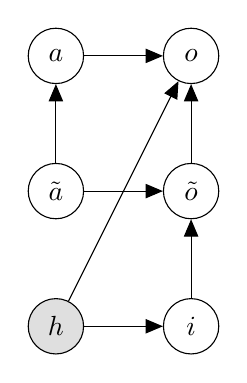
\begin{tikzpicture}
\node[obs] (h) {$h$};
\node[latent, right=of h] (i) {$i$};
\node[latent, above=of i] (to) {$\tilde{o}$};
\node[latent, above=of h] (ta) {$\tilde{a}$};
\node[latent, above=of to] (o) {$o$};
\node[latent, above=of ta] (a) {$a$};
\edge {h} {i};
\edge {h} {o};
\edge {i} {to};
\edge {ta} {a};
\edge {ta} {to};
\edge {to} {o};
\edge {a} {o};
\end{tikzpicture}
\end{center}
\item Abstract observation $\tilde{o} \bigCI h \mid \tilde{a}, i$
\end{itemize}
\end{frame}

\begin{frame}
\frametitle{Experiments}
\begin{itemize}
\item Mutual Friends
    \begin{itemize}
    \item Augment rule-based (prior work) to optimize info gain
    \item After OneCommon: Add neural on top
    \end{itemize}
\item OneCommon
    \begin{itemize}
    \item Use attributes = raw mention configurations
        \begin{itemize}
        \item Need belief / info gain / LR weights
        \item How to deal with redundancy? (i.e. correlation between features)
        \end{itemize}
    \item Learn latent refinement on top of mention configurations
    \end{itemize}
\end{itemize}
\end{frame}

\begin{frame}
\frametitle{Information gain issues}
\begin{itemize}
\item Best info gain could be to ask the same question twice
\item Usual fix: Limit to asking once only
\item Would be nice to have a principled way to deal with correlated
    features though
\end{itemize}
\centering
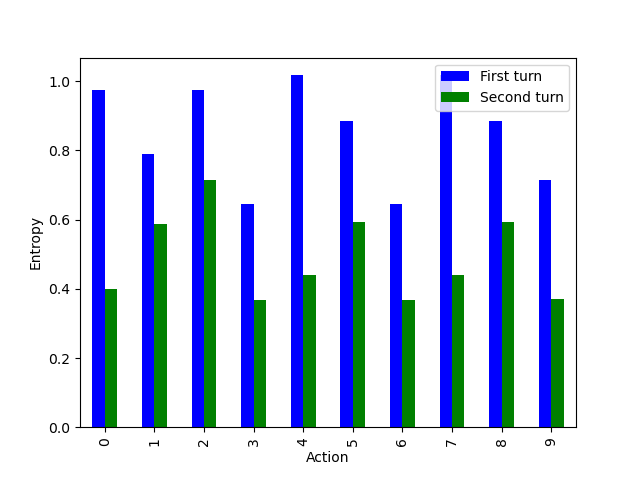
\includegraphics[height=2in]{src/entropy.png}
\begin{itemize}
\item Second turn after taking action with lowest entropy
\end{itemize}
\end{frame}

\begin{frame}
\frametitle{Related work: 20 questions}
\begin{itemize}
\item \citet{padmakumar}
    \begin{itemize}
    \item Attribute-based classification (string heuristic to map to description)
        + activate learning about attributes
    \item Info gain (on top of binary unweighted logistic regression) as feature for
        RL policy
    \end{itemize}
\item \citet{yu}
    \begin{itemize}
    \item Question-based classification (attributes)
    \item Learn weights of features
    \item Do not consider feature correlations
    \end{itemize}
\item More interesting language, symmetric setting
\item Learn weights, account for correlation
\item Symmetry, deal with unexpected features
\end{itemize}
\end{frame}

\begin{frame}
\frametitle{End}
\end{frame}


\begin{frame}
\frametitle{Concerns}
\begin{itemize}
\item Would a large LM solve all of this?
    \begin{itemize}
    \item Fine tune on small onecommon dataset, are there still repeats?
    \item Unlikely to solve strategy / over optimistism
    \end{itemize}
\end{itemize}
\end{frame}

\begin{frame}
\frametitle{End}
\end{frame}


\begin{frame}
\frametitle{Expected Information Gain}
\begin{align*}
IG(h, a) &= H(i \mid h) - \Es{p(o\mid h,a)}{H(i \mid h, a, o)}\\
\Es{p(o\mid h,a)}{H(i \mid h, a)} &= \sum_o\sum_{i'}p(o\mid h,a,i)p(i\mid h)H(i \mid h,a,o)
\end{align*}
\begin{itemize}
\item Equivalent to minimizing expected uncertainty after receiving a response
\item Cite Yu et al, White et al
\end{itemize}
\end{frame}

\begin{frame}[allowframebreaks]
\frametitle{Citations}
%\printbibliography
\bibliography{bib.bib}
\end{frame}

\begin{frame}
\frametitle{Games}

\begin{columns}
\begin{column}{0.5\textwidth}
\centering
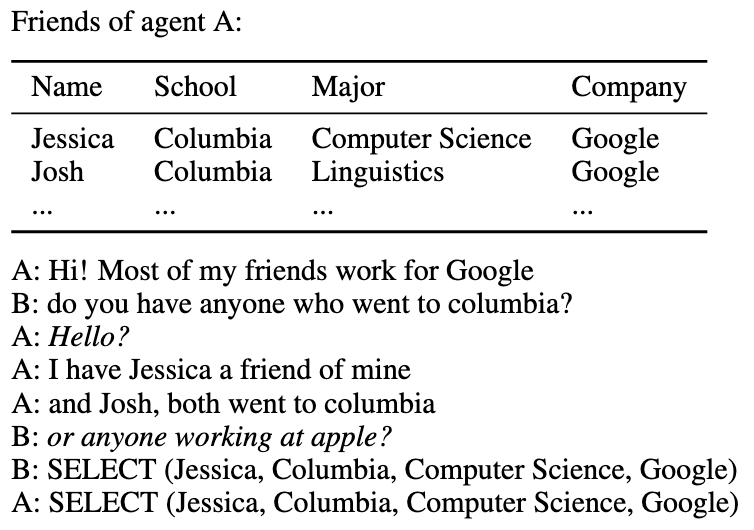
\includegraphics[width=2in]{img/mf.png}
\end{column}
\begin{column}{0.5\textwidth}
\centering
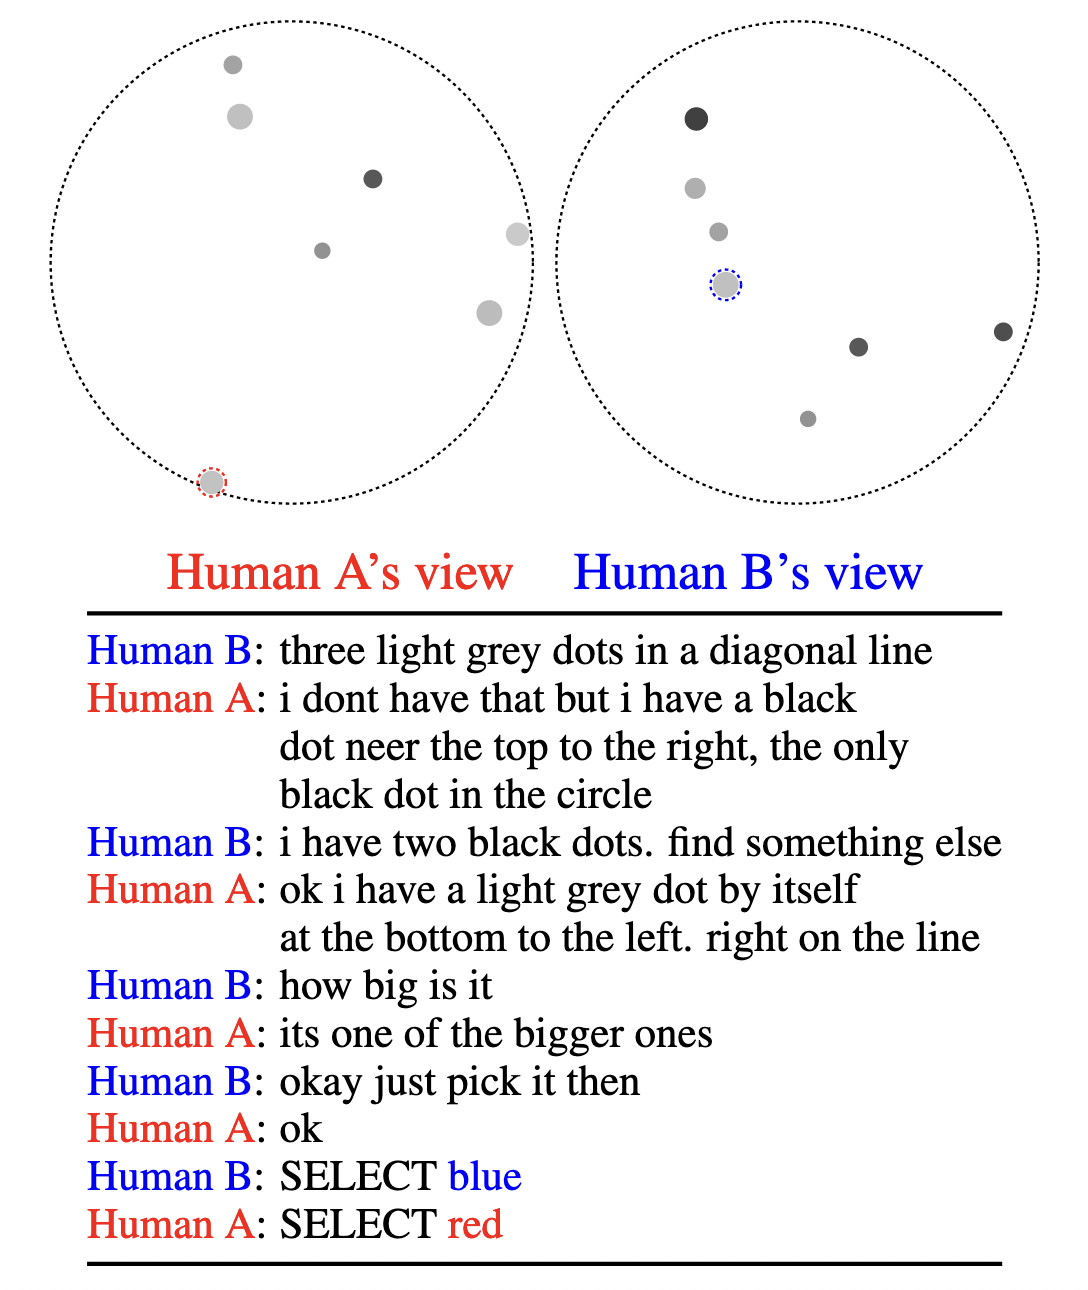
\includegraphics[width=2in]{img/oc.png}
\end{column}
\end{columns}

\vspace{2em}
\centering
Mutual Friends and OneCommon
\end{frame}

\begin{frame}
\frametitle{Issue: Poor neural reasoning}
From Mutual Friends: Neural + Human
\begin{itemize}
\item A: Know anyone who likes chess?
\item B: None of my friends like chess.
\item (conversation continues)
\item A: Crocheting?
\item B: None like crocheting.
\item A: Chess?
\item B: None like chess either, haha.
\end{itemize}
\end{frame}

\begin{frame}
\frametitle{Sample of prior work in model-based planning}
\begin{itemize}
\item 20 questions \citep{yu,padmakumar}
    \begin{itemize}
    \item Sym: Assymmetric questioner + answerer
    \item Turns: Multi-turn game
    \item Lang: Closed class answers (observations)
    \item Heur: Expected info gain heuristic
    \end{itemize}
\item EVPI \citep{rao,rao2}
    \begin{itemize}
    \item Sym: Assymmetric questioner + answerer
    \item Turns: No interaction, single turn game
    \item Lang: Open
    \item Heur: Expected utility heuristic
    \end{itemize}
\item RSA reference game \citep{khani}
    \begin{itemize}
    \item Sym: Symmetric
    \item Turns: Multi-turn game
    \item Lang: Symbolic language
    \item Heur: Bounded depth search
    \end{itemize}
\end{itemize}
\end{frame}

\begin{frame}
\frametitle{Conditioning in partner modeling}
\begin{itemize}
\item Assuming conditional independence $p(o \mid h, a, y) = p(o \mid a, y)$ is harmful
\item If you ask the same question twice, your belief changes both times!
    \begin{itemize}
    \item $p(\text{yes} \mid h = \emptyset, a=\text{red dot?},y)$ can vary depending on the latent $y$
    \item $p(\text{yes} \mid h = (\text{red dot?}, \text{yes}), a = \text{red dot?},y) = 1$,
        since we just asked!
    \end{itemize}
\item `Questions with correlated answers' and deficient observation model
    lead to uncalibrated beliefs, and therefore poor strategy
\item Contribution: relax independence assumption
    \begin{itemize}
    \item Let past obs vote on current one (weighted by action similarity)
    \item Probably solved by Transformers\footnote{Copy attention,
        depends on amount of data}
    \end{itemize}
\end{itemize}
\end{frame}

\begin{frame}
\frametitle{Example dialogue 1: Overconfidence}
\centering
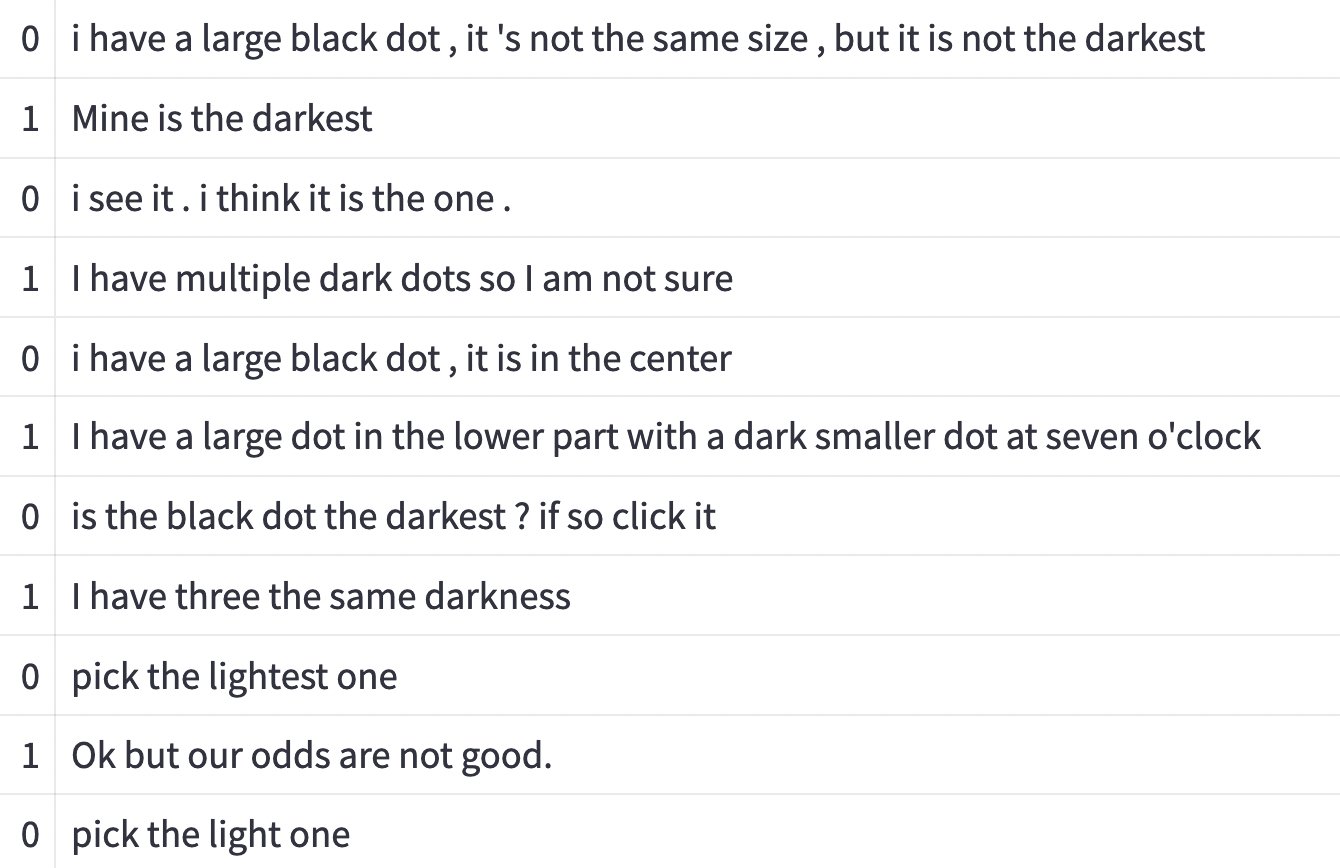
\includegraphics[width=\textwidth]{img/words1.png}
\end{frame}

\begin{frame}
\frametitle{Example dialogue 2: Overconfidence}
\centering
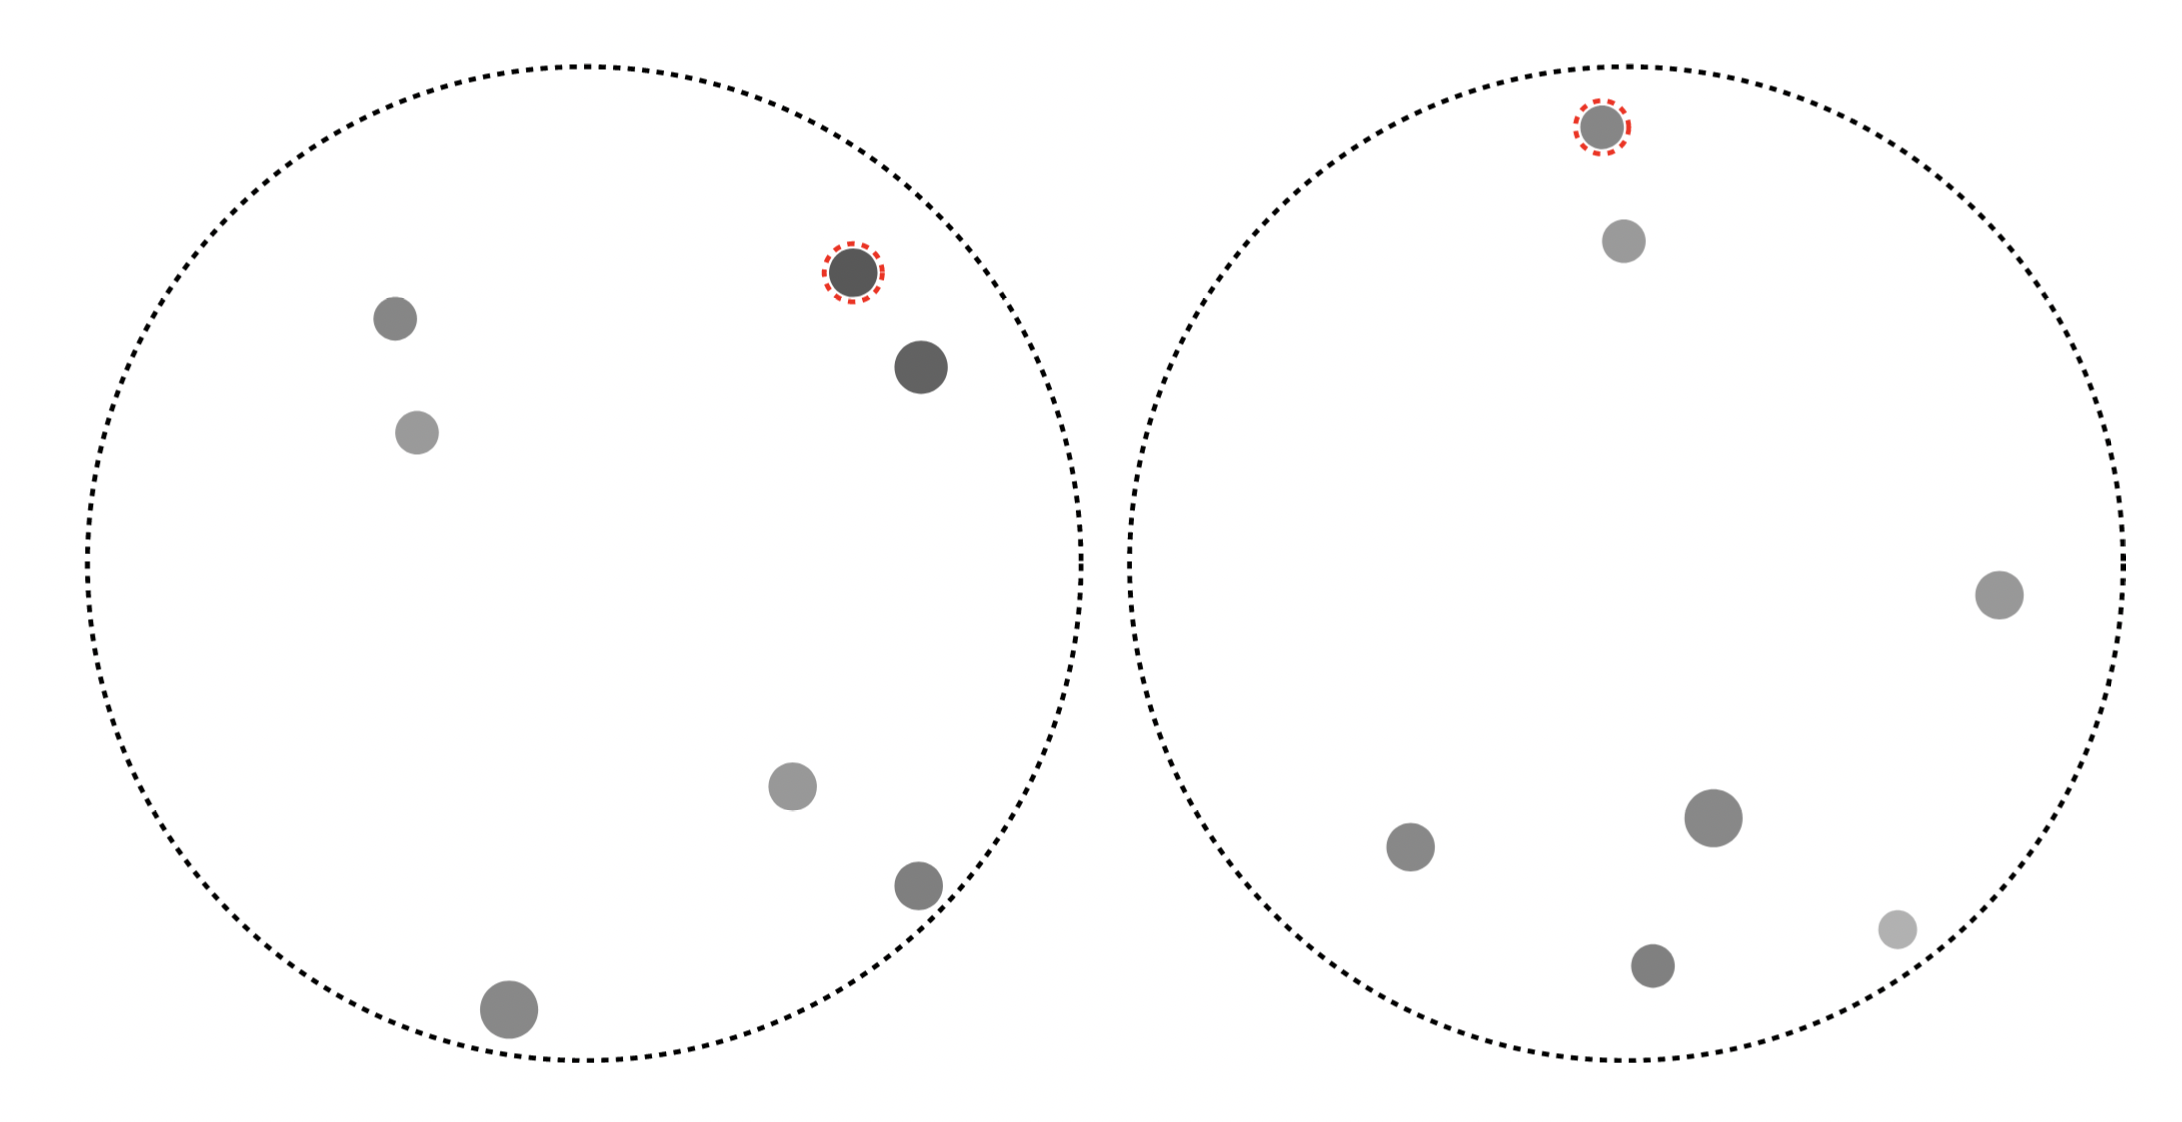
\includegraphics[width=0.75\textwidth]{img/dots2.png}
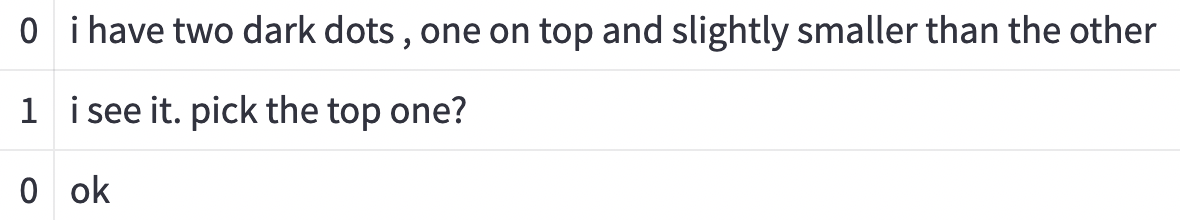
\includegraphics[width=\textwidth]{img/words2.png}
\end{frame}

\begin{frame}
\frametitle{Example dialogue 3: Good humans}
\centering
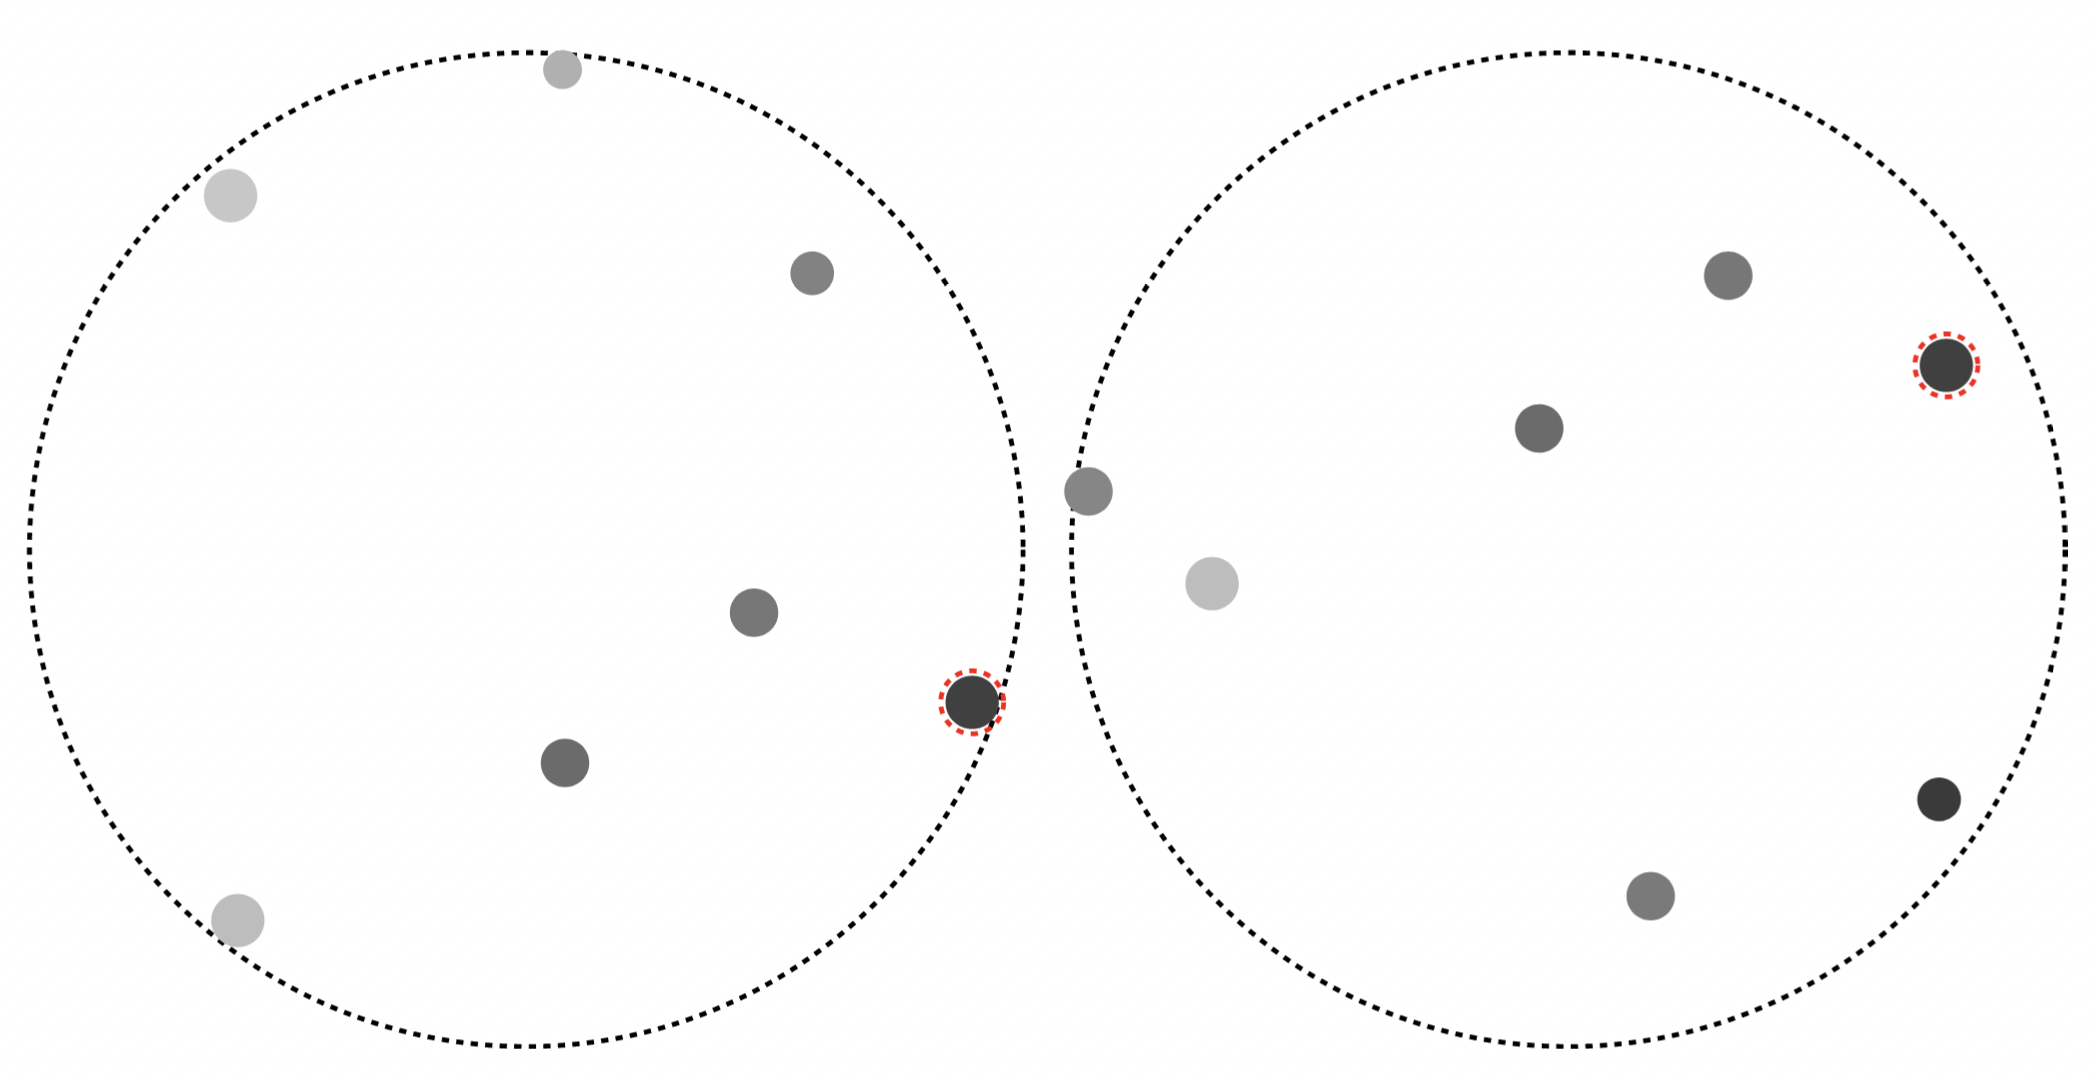
\includegraphics[width=0.75\textwidth]{img/dots3.png}
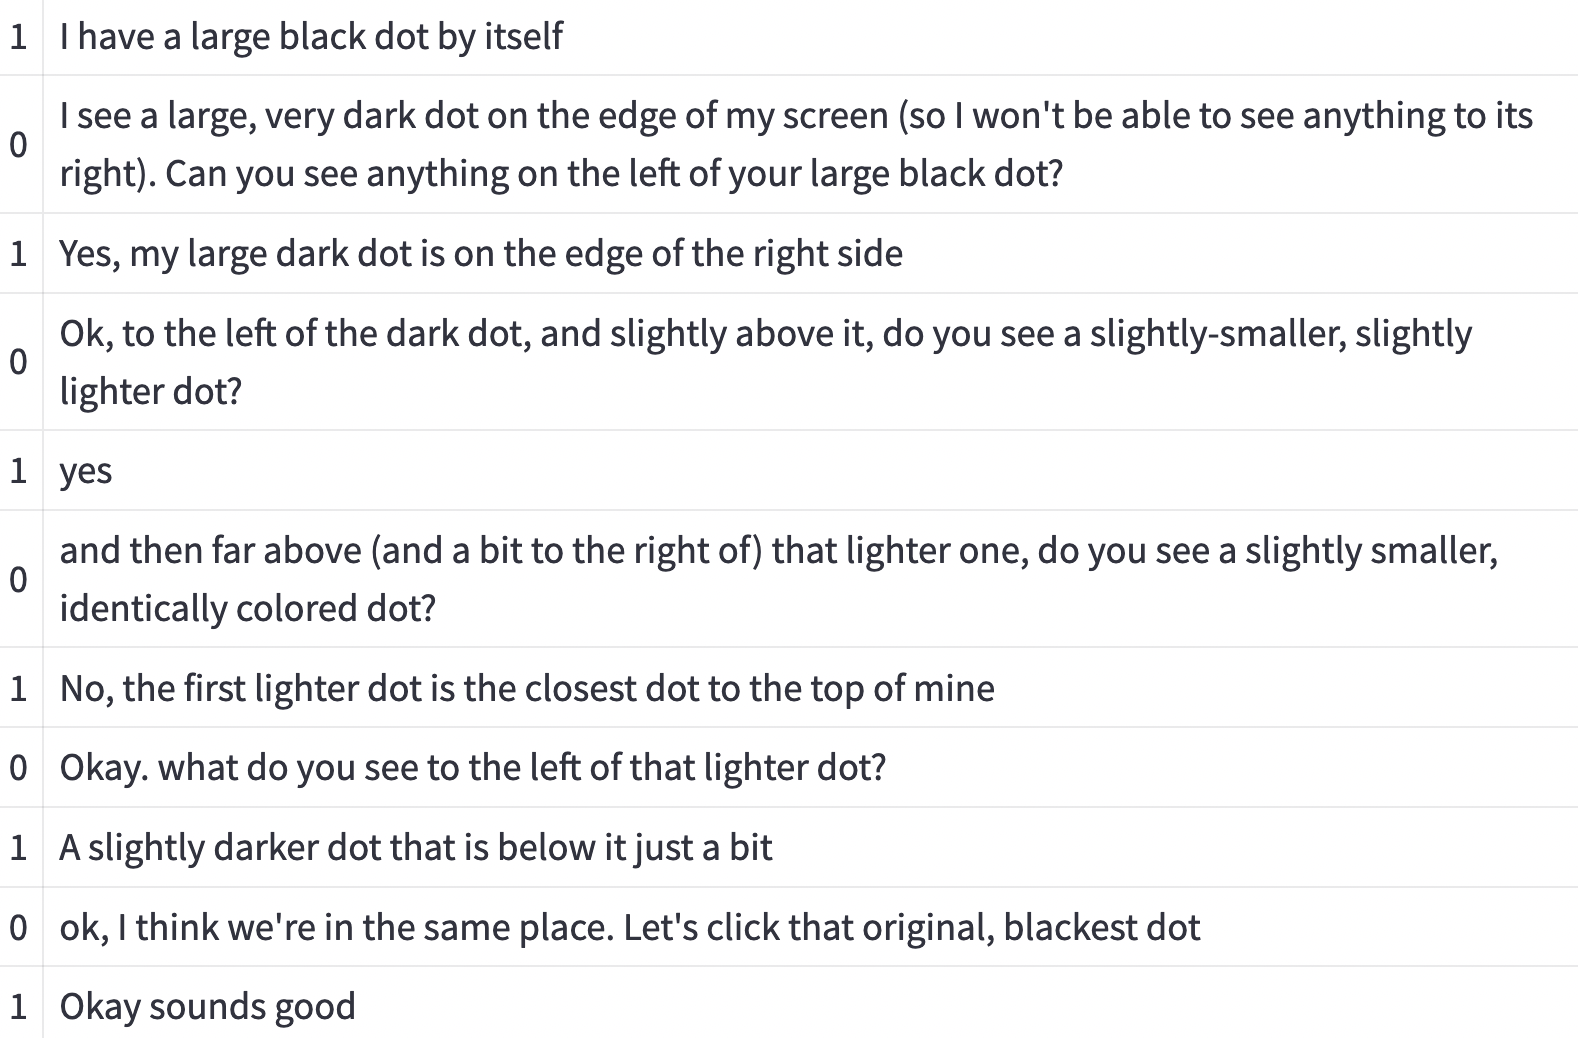
\includegraphics[width=\textwidth,clip,trim={0 9cm 0 0}]{img/words3.png}
\end{frame}

\begin{frame}
\frametitle{Example dialogue 3: Good humans}
\centering
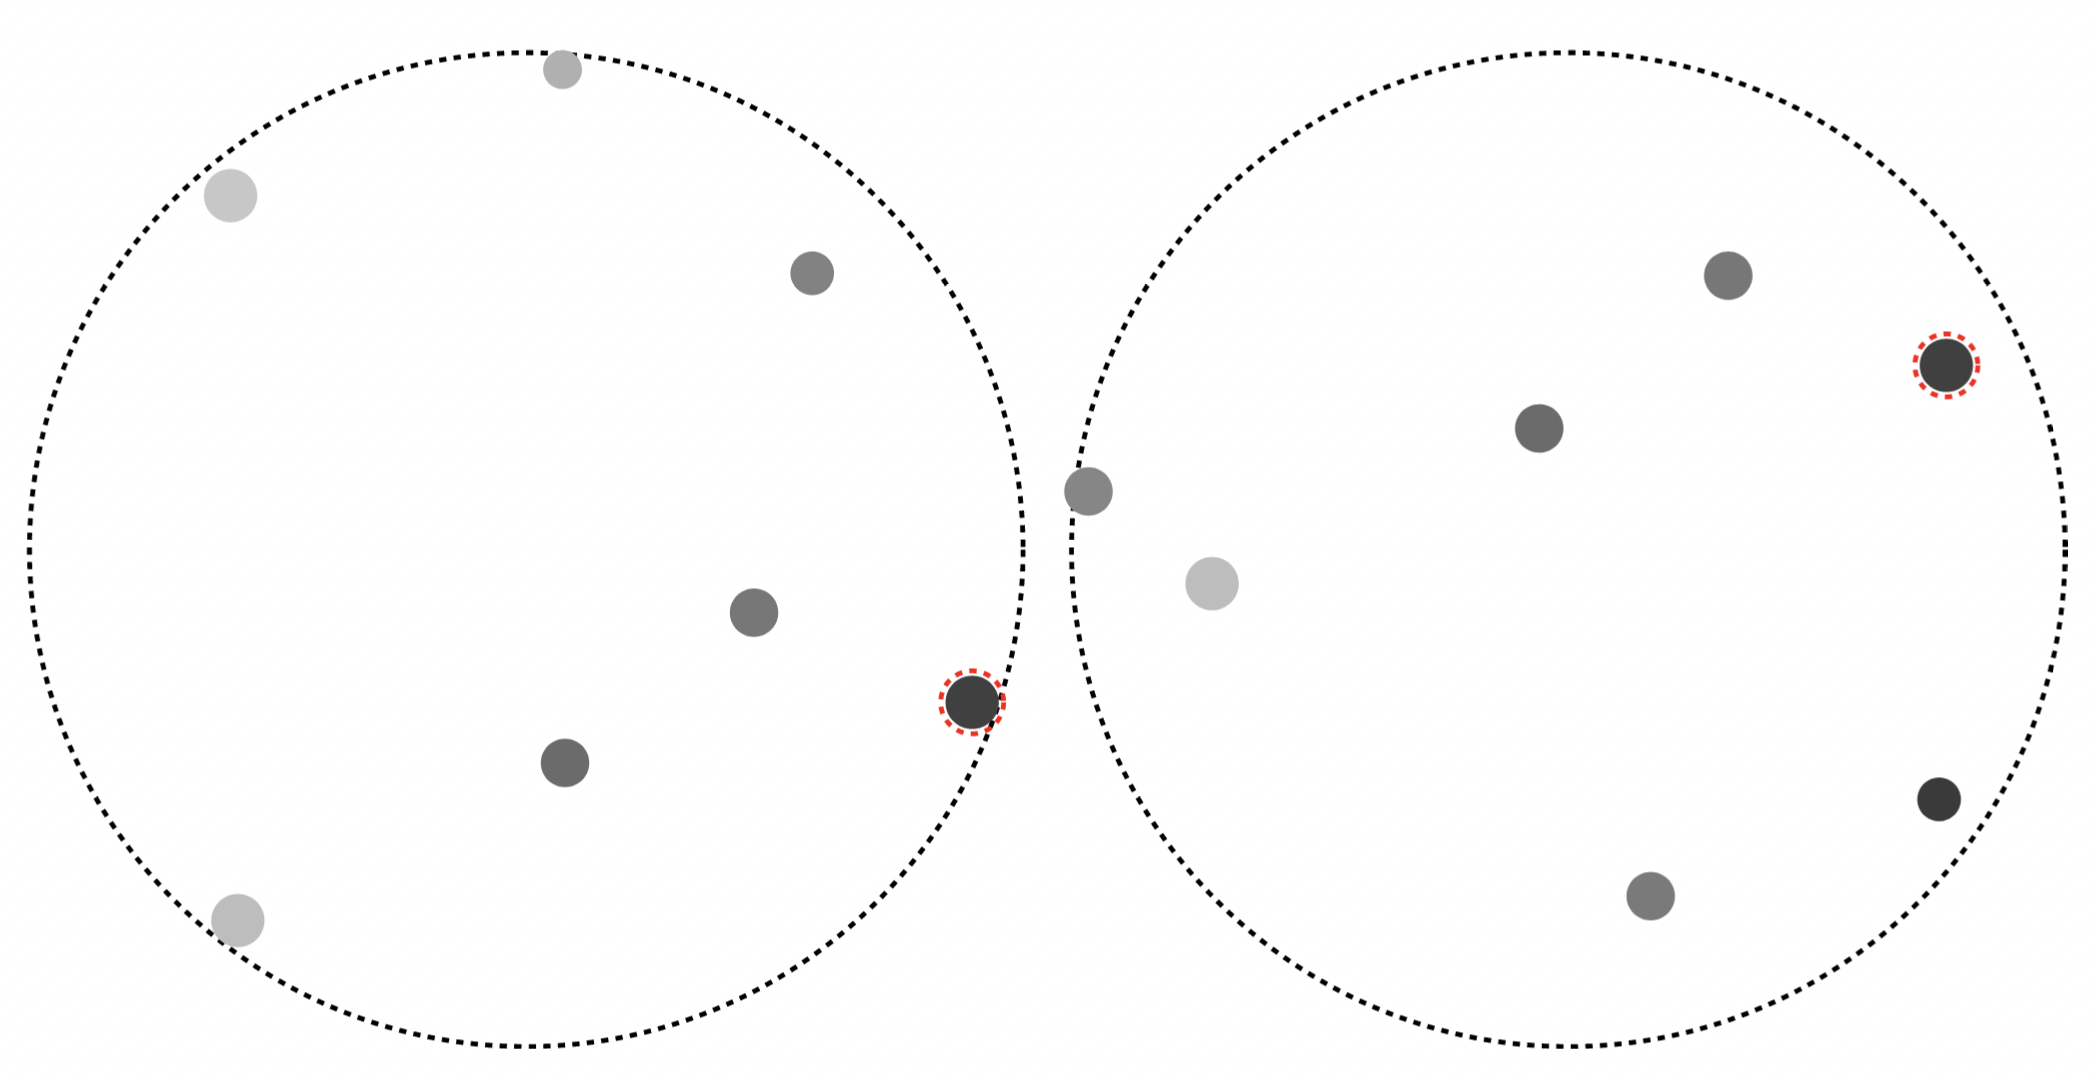
\includegraphics[width=0.75\textwidth]{img/dots3.png}
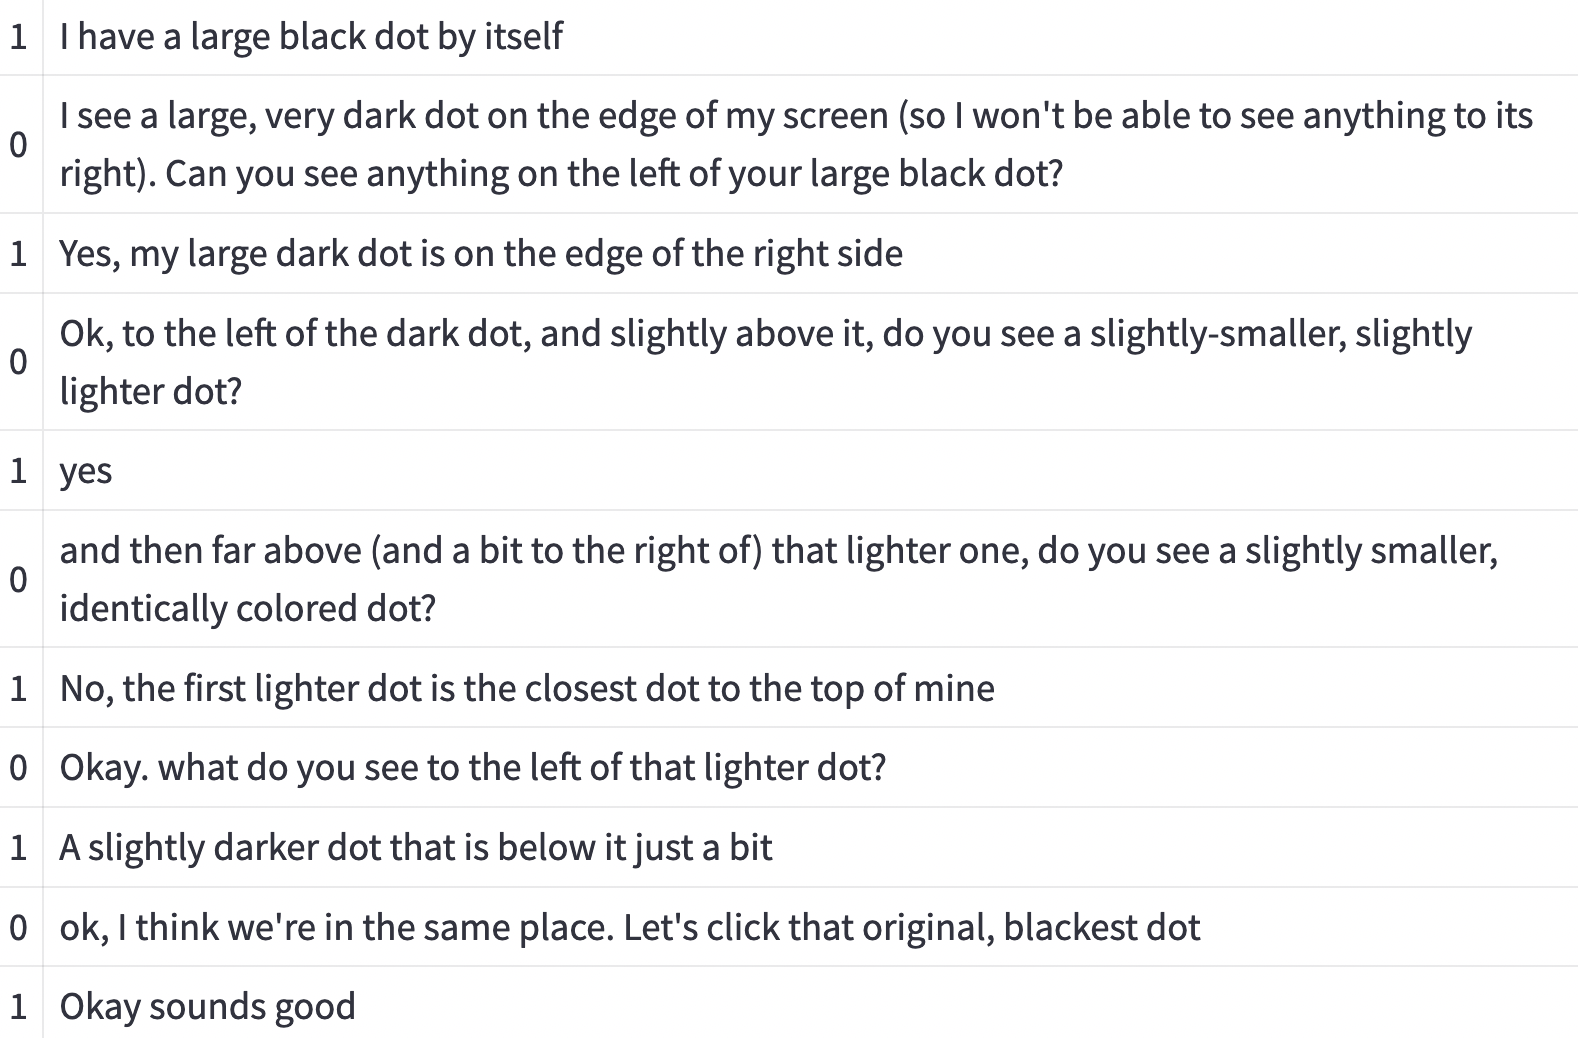
\includegraphics[width=\textwidth,clip,trim={0 0 0 9cm}]{img/words3.png}
\end{frame}



\end{document}
